\documentclass[11pt]{article}
\usepackage[UTF8]{ctex}
\usepackage[a4paper]{geometry}
\geometry{left=2.0cm,right=2.0cm,top=2.5cm,bottom=2.5cm}

\usepackage{caption}
\usepackage{paralist}
\usepackage{enumitem}
\setenumerate[1]{itemsep=0pt,partopsep=0pt,parsep=0pt,topsep=0pt}
\setitemize[1]{itemsep=0pt,partopsep=0pt,parsep=0pt,topsep=0pt}
\usepackage{comment}
\usepackage{booktabs}
\usepackage{graphicx}
\usepackage{float}
\usepackage{diagbox}
\usepackage{amsmath,amsfonts,graphicx,amssymb,bm,amsthm}
\usepackage{algorithm,algorithmicx}
% \usepackage[ruled, linesnumbered]{algorithm2e}
% \usepackage[linesnumbered]{algorithm2e}
\usepackage[noend]{algpseudocode}
\usepackage{fancyhdr}
\usepackage{tikz}
\usepackage{graphicx}
\usetikzlibrary{arrows,automata,positioning}
\usepackage{hyperref}
\usepackage{extarrows}
% 这是一些字体选项
\usepackage{helvet}
% \usepackage{mathpazo}
\usepackage{fontspec}
% \setmainfont{Times New Roman}
% \setmainfont{Comic Sans MS} % 比较fancy的字体
% \setmainfont{Avenir}
% \setmainfont{Palatino}

\setlength{\headheight}{14pt}
\setlength{\parindent}{0 in}
\setlength{\parskip}{0.5 em}


\newtheorem{theorem}{Theorem}
\newtheorem{lemma}[theorem]{Lemma}
\newtheorem{proposition}[theorem]{Proposition}
\newtheorem{claim}[theorem]{Claim}
\newtheorem{corollary}[theorem]{Corollary}
\newtheorem{definition}[theorem]{Definition}
\newtheorem*{definition*}{Definition}

\newenvironment{problem}[2][Problem]{\begin{trivlist}
\item[\hskip \labelsep{\bfseries#1}\hskip\labelsep{\bfseries#2.}]}{\hfill$\blacktriangleleft$\end{trivlist}}
\newenvironment{answer}[1][Answer]{\begin{trivlist}
\item[\hskip \labelsep{\bfseries\itshape#1.}\hskip \labelsep]}{\hfill$\lhd$\end{trivlist}}

\newcommand\E{\mathbb{E}}
\newcommand\per{\mathrm{per}}
\renewcommand{\algorithmicrequire}{\textbf{Input:}}
\renewcommand{\algorithmicensure}{\textbf{Output:}}
\algrenewcommand{\algorithmiccomment}[1]{\hfill $//$ #1}
% chktex-file 44
% \renewcommand{\familydefault}{\sfdefault}

\RequirePackage{algorithm}

\makeatletter
\newenvironment{breakablealgorithm}
  {% \begin{breakablealgorithm}
    \begin{center}
      \refstepcounter{algorithm}% New algorithm
      \hrule height.8pt depth0pt \kern2pt% \@fs@pre for \@fs@ruled
      \parskip 0pt
      \renewcommand{\caption}[2][\relax]{% Make a new \caption
        {\raggedright\textbf{\fname@algorithm~\thealgorithm} ##2\par}%
        \ifx\relax##1\relax % #1 is \relax
          \addcontentsline{loa}{algorithm}{\protect\numberline{\thealgorithm}##2}%
        \else % #1 is not \relax
          \addcontentsline{loa}{algorithm}{\protect\numberline{\thealgorithm}##1}%
        \fi
        \kern2pt\hrule\kern2pt
     }
  }
  {% \end{breakablealgorithm}
     \kern2pt\hrule\relax% \@fs@post for \@fs@ruled
   \end{center}
  }
\makeatother

% set for automata
\tikzset{>=stealth',shorten >=1pt,auto,node distance=2cm, % Increase node distance to 4cm
                    thick,main node/.style={circle,draw,font=\sffamily\Large\bfseries}}


\title{Homework \#4}
\usetikzlibrary{positioning}

\begin{document}
\captionsetup[figure]{labelfont={bf},name={Fig.},labelsep=period}
\kaishu

\pagestyle{fancy}
\lhead{\CJKfamily{zhkai} Peking University}
\chead{}
\rhead{\CJKfamily{zhkai} Algorithm Design and Analysis (Honor Track)}

\begin{center}
    {\LARGE \bf Homework 4}\\
    {Name: 方嘉聪\ \  ID: 2200017849}            % Write down your name and ID here.
\end{center}

\textbf{$\bullet$~NOTE: } We will refer to \textbf{design an algorithm, prove its correctness and analyze the running time} as a \textbf{3-part solution}.

\begin{problem}{1 (Occupied Scheduling)}
    You are given a set of $m$ time intervals $[s_i, f_i]$, where $1\leqslant i\leqslant m$. You are also given a set of $n$ possible events
    with times $T=\{t_1,t_2,\ldots,t_n\}$. We say that an event $j$ hits an interval $i$ if this event time lies within the interval, that is, $t_j\in[s_i,f_i]$. It is assumed that every interval is hit by at least one event.
    
    Present a \textbf{polynomial-time} algorithm to determine a set of events from $T$ with the minimum number of events such that the events in the set hit every one of the intervals. \textbf{Please give a 3-part solution}.

\end{problem}
\begin{answer}
这题我们用事件“覆盖”区间表示\textbf{hit}. \\
基本思路: 先将事件按照时间升序排序得到$T' = \{t_1^*, t_2^*, \cdots, t_n^* \}$.设$S$为一个新的区间集, 遍历每个区间$[s_i, f_i]$ 得到落在这一区间内的发生时间最早和最晚的时间点$t_{i,\min}$和$t_{i,\max}$, 将区间$[t_{i,\min}, t_{i,\max}]$加入$S$中(如果二者相等则退化为一个点, 不会影响后续分析).
而后将$S$按照左端点升序排序得到$S' = \{[t_{1,\min}, t_{1, \max}], [t_{2,\min}, t_{2, \max}], \cdots,[t_{m,\min}, t_{m, \max}]\}$, 而后按照从左到右的顺序不断对$S'$内的区间与其后续的区间取并集, 当前交集与后一个区间交为空说明对目前的事件已经覆盖了最多的时间区间, 将交集的端点加入结果集合$A$中, 从下个区间开始继续循环这一操作, 直至遍历整个$S$. 最后返回$A$即为所求的最小事件集合.
\\伪代码如下:
\begin{breakablealgorithm}
    \caption{\textbf{Occupied Scheduling}}
    \begin{algorithmic}[1]
        \Require $m$个区间$[s_i, f_i]$, $n$个事件时间$T$
        \Ensure 最小事件集合$A$和事件个数$num$
        \State 对$T$按照时间升序排序得到$T'$
        \State $S \leftarrow \emptyset$, $A \leftarrow \emptyset$, $num \leftarrow 0$
        \For{$i = 1$ to $m$}
            \State $t_{i,\min} \leftarrow \min\{t_j | t_j \in T \land t_j \in [s_i, f_i]\}$
            \State $t_{i,\max} \leftarrow \max\{t_j | t_j \in T \land t_j \in [s_i, f_i]\}$
            \State $S \leftarrow S \cup \{[t_{i,\min}, t_{i,\max}]\}$
        \EndFor
        \State 对$S$按照左端点升序排序得到$S'$
        \State $interval \leftarrow S'[0]$
        \For {$i \leftarrow 1$ to $m-1$}
            \If{$interval \cap S'[i] = \emptyset$}
                \State $A \leftarrow A \cup \{interval[0]\}$
                \State $interval \leftarrow S'[i]$
                \State $num \leftarrow num + 1$
            \Else
                \State $interval \leftarrow interval \cup S'[i]$
            \EndIf
        \EndFor
        \State $A \leftarrow A \cup \{interval[0]\}$, $num \leftarrow num + 1$
        \State \Return $A, num$
    \end{algorithmic}
\end{breakablealgorithm}
\textbf{时间复杂度分析:} 第1行和第7行的排序为$O(n \log n)$和$O(m \log m)$, 第3-6行的循环为$O(m \log n)$, 第8-16行的循环为$O(m)$, 故总时间复杂度为$O((m+n)\log (mn))$, 为多项式时间.
\\ \textbf{算法正确性证明:} 我们考虑最优解$\{t_{i_1}, t_{i_2}, \cdots, t_{i_a}\}$, 不妨设$t_{i_1} < t_{i_2} < \cdots < t_{i_a}$, 贪心算法得到的解为$\{t_{i_1}^*, t_{i_2}^*, \cdots, t_{i_a}^*\}$(不妨设为升序排序). 我们用数学归纳法对解的规模$k$进行证明贪心算法得到的事件集合所覆盖的区间不会小于最优解所覆盖的区间. 
\begin{itemize}
    \item 归纳奠基: 当$k = 1$时: 设$t_{i_1}$和$t_{i_1}^*$覆盖的区间集为$A_1 = \{[s_i, f_i]\}, A_{1}^* = \{[s_j, f_j]\}$. 若$A_{1}^* \subsetneq A_{1}$, 这与伪代码的第8-16行的循环矛盾(这个循环保证了只要一个区间与$A_{1}^*$中的区间的交有交集, 那么这一区间也会包含$t_{i_1}^*$), 故$A_1 \subseteq A_{1}^*$, 即贪心算法得到的解所覆盖的区间不会小于最优解所覆盖的区间. 
    \item 归纳假设: 假设当$k = s$时, 贪心算法的解覆盖的区间$\bigcup_{i=1}^{s}A_i$不会小于最优解所覆盖的区间$\bigcup_{i=1}^{s}A_i^*$. 
    \item 归纳步骤: 当$k = s + 1$时, 设$t_{i_{s+1}}$和$t_{i_{s+1}}^*$覆盖的区间集为$A_{s+1},A_{s+1}^*$, 类似归纳奠基的证明伪代码的8-16行的循环保证了$A_{s+1} \subseteq A_{s+1}^*$, 结合归纳假设有$\bigcup_{i=1}^{s+1}A_i \subseteq \bigcup_{i=1}^{s+1}A_i^*$.
\end{itemize}
综上, 贪心算法得到的事件集合所覆盖的区间不会小于最优解所覆盖的区间, 算法正确性得证.
\end{answer}
\begin{problem}{2 (Bottleneck of Spanning Trees)}
    Let $G=(V,E)$ be a connected graph with $n$ vertices, $m$ edges, and positive edge costs that you may assume are all \textit{distinct}. Let $G^{\prime}=(V,T)$ be a spanning tree of $G$; we define the \textit{bottleneck edge} of $G^{\prime}$ to be the edge in $T$ with the greatest cost. A spanning tree $G^{\prime}=(V,T)$ is a \textit{minimum-bottleneck spanning tree} if there is no other spanning tree of $G$ with a cheaper bottleneck edge.
\begin{enumerate}[label=(\arabic*)]
    \item Is every minimum-bottleneck spanning tree of $G$ a minimum spanning tree of $G$? Prove or give a counterexample.
    \item Is every minimum spanning tree of $G$ a minimum-bottleneck spanning tree of $G$? Prove or give a counterexample.
\end{enumerate}
\end{problem}
\begin{answer}

\begin{enumerate}[label=(\arabic*)]
    \item 考虑如下图,图$G_1$为$G$的最小瓶颈生成树但不是最小生成树.
    \begin{figure}[h]
        \begin{minipage}{0.5\textwidth}
        \centering
        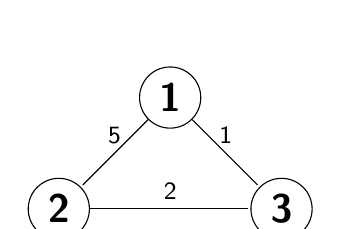
\begin{tikzpicture}
            \node[main node] (1) {1};
            \node[main node] (2) [below left of=1] {2};
            \node[main node] (3) [below right of=1] {3};

            \path[every node/.style={font=\sffamily\small}]
                (1) edge node [above] {5} (2)
                (1) edge node [above] {1} (3)
                (2) edge node [above] {2} (3);
        \end{tikzpicture}
        \caption{图$G$}
        \end{minipage}
        \begin{minipage}{0.5\textwidth}
        \centering
        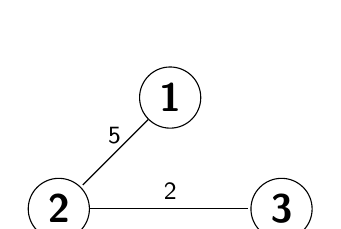
\begin{tikzpicture}
            \node[main node] (1) {1};
            \node[main node] (2) [below left of=1] {2};
            \node[main node] (3) [below right of=1] {3};

            \path[every node/.style={font=\sffamily\small}]
                (1) edge node [above] {5} (2)
                (2) edge node [above] {2} (3);
        \end{tikzpicture}
        \caption{图$G_1$}
        \end{minipage}
    \end{figure}
    \item 正确. 设$G_0 = (V, E_0)$为$G$的最小生成树, 如果存在一个生成树$G' = (V, T)$使得$G'$的最大边权小于$G_0$的最大边权. 设$G_0$中边权最大的边为$e_{\max}$, 我们去掉$e_{\max}$使得$G_0$被割为两个不连通的部分$V_1$和$ V_2$. 那么在$T$中$\exists e = (u, v), ~s.t.~ u \in V_1, v \in V_2$, 且$cost(e_{\max}) > cost(e)$. 考虑$G^* = (V, (E_0 \backslash \{e_{\max}\}) \cup \{e\} )$, 那么$G^*$的边权和小于$G_0$这与$G_0$为最小生成树矛盾. 故$G_0$为最小瓶颈生成树.
\end{enumerate}

\end{answer}

\begin{problem}{3 (Minimum Spanning $k$-Forest)}
    Given a graph $G=(V, E)$ with nonnegative weights, a spanning $k$-forest is a cycle-free collection of edges $F \subseteq E$ such that the graph with the same vertices as $G$ but only the edges in $F$ has $k$ connected components. For example, consider a fully connected graph $G=(V, E)$ with vertices $V=\{A, B, C, D, E\}$. One spanning 2-forest of this graph is $F=$ $\{(A, C),(B, D),(D, E)\}$, because the graph with vertices $V$ and edges $F$ has components $\{A, C\},\{B, D, E\}$

    The minimum spanning $k$-forest is defined as the spanning $k$-forest with the minimum total edge weight. (Note that when $k=1$, this is equivalent to the minimum spanning tree). In this problem, you will design an algorithm to find the minimum spanning $k$-forest. For simplicity, you may assume that all edges in $G$ have \textit{distinct} weights. 
    \begin{enumerate}[label=(\arabic*)]
        \item Define a $j$-partition of a graph $G$ to be a partition of the vertices $V$ into $j$ (non-empty) sets. That is, a $j$-partition is a list of $j$ sets of vertices $\Pi=\left\{S_{1}, S_{2} \ldots S_{j}\right\}$ such that every $S_{i}$ includes at least one vertex, and every vertex in $G$ appears in \textbf{exactly one} $S_{i}$. For example, if the vertices of the graph are $\{A, B, C, D, E\}$, one 3-partition is to split the vertices into the sets $\Pi=\{\{A, B\},\{C\},\{D, E\}\}$. Define an edge $(u, v)$ to be crossing a $j$-partition $\Pi=\left\{S_{1}, S_{2} \ldots S_{j}\right\}$ if the set in $\Pi$ containing $u$ and the set in $\Pi$ containing $v$ are different sets. For example, for the 3-partition $\Pi=\{\{A, B\},\{C\},\{D, E\}\}$, an edge from $A$ to $C$ would cross $\Pi$. \textbf{Prove that for any $j$-partition $\Pi$ of a graph $G$, if $j>k$ then the lightest edge crossing $\Pi$ must be in the minimum spanning $k$-forest of $G$}.
        \item Give an efficient algorithm for finding the minimum spanning $k$-forest. \textbf{Please give a 3-part solution}.
    \end{enumerate}
\end{problem}
\begin{answer}
    \begin{enumerate}[label = (\arabic*)]
        \item 设$\Pi = \{S_1, S_2, \cdots, S_j\}$,边$e_{\min} = (u, v)$为跨越$\Pi$的最小权边, $G$的最小$k$-生成森林中为$F = \{E_1, E_2, \cdots\, E_k\}$.假设$e_{\min} \not\in F$, 我们分两种情况讨论:
        \begin{itemize}
            \item 若$\exists~ E_t \in F ~s.t.~ u, v \in E_t$, 那么在$E_t$中一定存在一条边$e'$跨越了$\Pi$, 根据$e_{\min}$的定义, cost($e_{\min}$) $\leq$ cost($e'$). 考虑$E_t - e' + e_{\min}$那么在$F$中的总权值会减小, 这与$F$为最小生成森林矛盾.
            \item 若$\exists~ E_{t_1} \text{ and } E_{t_2}(t_1 \neq t_2), ~s.t.~ u \in E_{t_1}, v \in E_{t_2}$. 我们将$e_{\min}$添加到$F$中, 这会导致$F$中的连通分量数量变为$k - 1$. 由于$j > k$, 那么存在边$e_0 \in F$且$e_0$跨越了$\Pi$, 我们把$e_0$从$F$中移除. 那么$F - e_0 + e_{\min}$的总权重会减小, 这与$F$为最小生成森林矛盾.
        \end{itemize} 
        综上, 跨越$\Pi$的最小权重边一定在$G$的最小$k$-生成森林中.
        \item 设$|V| = n, |E| = m$. 算法思路: 类似Kruskal算法, 使用并查集, 初始化每个点作为一个partition, 先将边按照权重排序, 而后从小到大遍历每条边, 如果边的两个端点不在同一个partition中, 则将这条边加入到生成森林中, 并将这两个partition合并. 当生成森林中的连通分量数为$k$时停止. 伪代码如下:
        \begin{breakablealgorithm}
            \caption{\textbf{Minimum Spanning $k$-Forest's Kruskal Algorithm}}
            \begin{algorithmic}[1]
                \Require $G = (V, E)$, $k$
                \Ensure $F$为$G$的最小$k$-生成森林
                \State 对$E$按照权重升序排序得到$E'$
                \State $F \leftarrow \emptyset$, $num \leftarrow 0$, $i \leftarrow 0$
                \State 初始化并查集$U$
                \For{$i = 1$ to $n$}
                    \State $U$.MakeSet($v_i$)
                \EndFor
                \While{$num < k$}
                    \State $e = E'[i]$
                    \If{$U$.Find($e.u$) $\neq U$.Find($e.v$)}
                        \State $F \leftarrow F \cup \{e\}$
                        \State $U$.Union($e.u, e.v$)
                        \State $num \leftarrow num + 1$
                    \EndIf
                    \State $i \leftarrow i + 1$
                \EndWhile
                \State \Return $F$
            \end{algorithmic}
        \end{breakablealgorithm}
        \begin{itemize}
            \item 时间复杂度分析: 与Kruskal算法相同, 排序的时间复杂度为$O(m \log m)$, 并查集的操作时间复杂度为$O(m \alpha(m, n)) = O(m \log m)$, 由于$m < n^2 \implies \log m = O(\log n)$, 故总时间复杂度为$O(m \log n)$.
            \item 算法正确性证明: 根据$(1)$的证明, 我们知道跨越$\Pi$的最小权重边一定在最小$k$-生成森林中, 算法保证了每次添加进$F$中一定是权重最小的跨越边(即在最小$k$-生成森林中),当算法停止时恰有$k$个连通分量, 即为最小$k$-生成森林. 算法正确性得证.
        \end{itemize}
    \end{enumerate}
\end{answer}

\begin{problem}{4 (Clock Tree Synthesis)}
    In the design automation of VLSI chips, timing circuits are crucial components. Consider the following model of clock tree synthesis (CTS), given a complete binary tree with $n$ leaves, where $n$ is a power of two. Each edge $e$ of the tree has an associated, positive length $l_e$. The \textit{distance} from the root to a given leaf is the sum of the lengths of all the edges on the path from the root to the leaf.
    
    The root generates a \textit{clock signal} which is propagated along the edges to the leaves. We assume that the time it takes for the signal to reach a given leaf is proportional to the distance from the root to the leaf. In realistic circuits, the distance is the net delay caused by parasite resistance/capacitance (RC), and the leaves represent sequential logic instances (e.g., flip-flops), which must be completely \textit{synchronized}, i.e., all should receive the clock signal at the same time. To make this happen, we will have to increase the lengths of certain edges, so that all root-to-leaf paths have the same length (we’re not able to shrink edge lengths). If we achieve this, then the tree (with its new edge lengths) will be said to have \textit{zero skew}. Our goal is to achieve zero skew in a way that keeps the sum of all the edge lengths as small as possible.

    Give an algorithm that increases the lengths of certain edges so that the resulting tree has zero skew and the total edge length is as small as possible. \textbf{Please give a 3-part solution.}

    \textbf{Example.} Consider the tree in Fig. \ref{fig1}, in which letters name the nodes and numbers indicate the edge lengths. The unique optimal solution for this instance would be to take the three length-1 edges and increase each of their lengths to $2$. The resulting tree has zero skew, and the total edge length is $12$, the smallest possible.

    \begin{figure}[H]
        \centering
        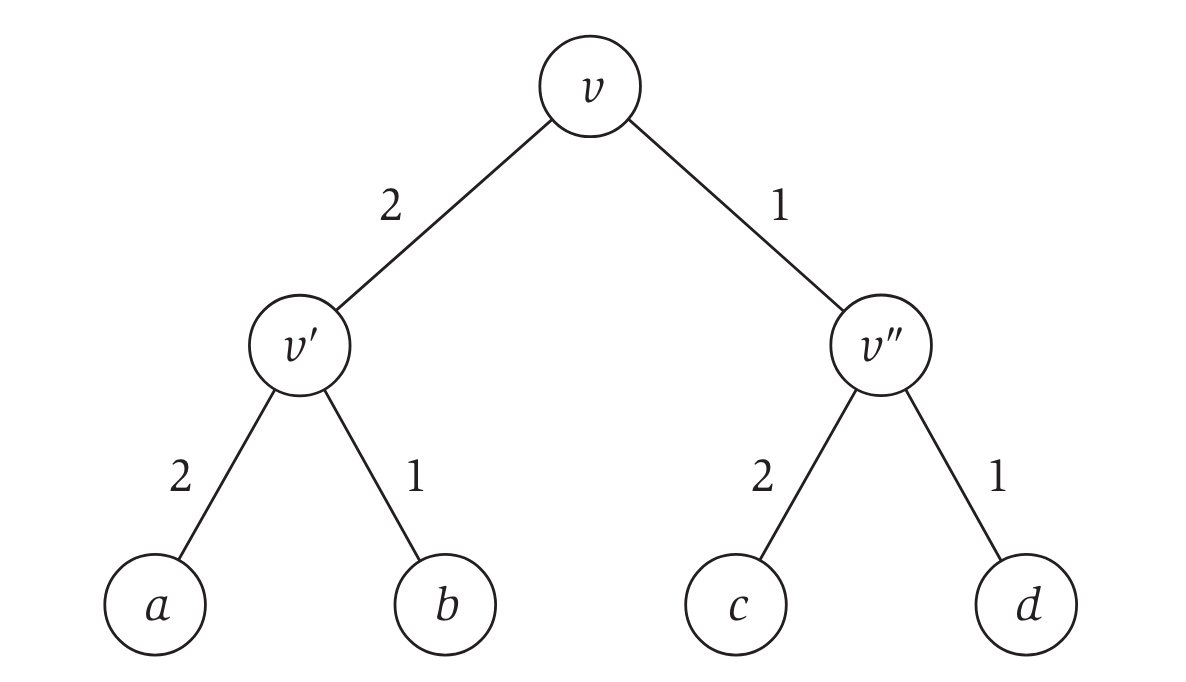
\includegraphics[width=0.5\textwidth]{iamge/cts.png}
        \caption{An instance of the zero-skew CTS problem.}
        \label{fig1}
    \end{figure}
\end{problem}
\begin{answer}
    算法思路: 设根节点为$v$, 左右子节点分别为$v_{l}, v_{r}$, 设$v-v_l-\text{leaf}$, $v - v_r - \text{leaf}$的最大距离分别为$dis_{l}, dis_{r}$. 
    \begin{itemize}
        \item 如果$dis_l = dis_r$, 则不需要修改$len(v, v_l), len(v, v_r)$. 递归的处理$v_l, v_r$.
        \item 如果$dis_l > dis_r$, 则令$len(v, v_r) = len(v, v_r) + dis_l - dis_r$. 递归的处理$v_l, v_r$.
        \item 如果$dis_l < dis_r$, 则令$len(v, v_l) = len(v, v_l) + dis_r - dis_l$. 递归的处理$v_l, v_r$.
    \end{itemize}
    伪代码如下:
    \begin{breakablealgorithm}
        \caption{\textbf{Zero-skew CTS}}
        \begin{algorithmic}[1]
            \Require 树$T = (V, E)$, $v$为根节点
            \Ensure 满足zero-skew的树$T'$和最小总边长$total$
            \State $total \leftarrow 0$
            \Function{DFS}{$v$}
                \If{$v$为叶子节点}
                    \State \Return $0$
                \EndIf
                \State $dis_l \leftarrow \text{DFS}(v_l)$, $dis_r \leftarrow \text{DFS}(v_r)$
                \If{$dis_l > dis_r$}
                    \State $len(v, v_r) \leftarrow len(v, v_r) + dis_l - dis_r$
                    \State $total \leftarrow total + dis_l - dis_r$
                \ElsIf{$dis_l < dis_r$}
                    \State $len(v, v_l) \leftarrow len(v, v_l) + dis_r - dis_l$
                    \State $total \leftarrow total + dis_r - dis_l$
                \EndIf
                \State \Return $\max(dis_l, dis_r) + len(v, v_l) + len(v, v_r)$
            \EndFunction
            \State \Return \textsc{DFS}($v$)
        \end{algorithmic}
    \end{breakablealgorithm}
    \begin{itemize}
        \item 算法复杂性分析: 树的叶子结点数为$n$, 算法的时间复杂度为$O(n)$.
        \item 算法正确性证明: 设$T^*, T$分别为最优解与贪心算法得到的解, 我们用交换论证来证明贪心算法得到的是唯一的最优解.首先先来证明关于最优解的两个引理:
        \begin{lemma}
            \songti
            设$w$为$T^*$的一个内部节点(非根节点), 如果$w$与其左右子节点相连的边$w_l, w_r$的长度都增加了, 则$T^*$不是最优解.
        \end{lemma}
        \begin{proof}
            \kaishu
            设$(w, w_l), (w, w_r)$的长度分别增加了$\delta_l, \delta_r$, 不妨设$\delta_l \ge \delta_r$. 考虑$w$的父节点$w_p$, 我们令$(w_p, w)$的长度增加$\delta_r$, $(w, w_l), (w, w_r)$的长度都减小$\delta_r$, 得到$T'$, 显然$T'$满足zero-skew, 且$T'$的总边长小于$T^*$, 这与$T^*$为最优解矛盾.
        \end{proof}
        \begin{lemma}
            \songti
            设$w$为$T^*$的非根或叶子的节点, 如果每条从$w$到$w$下所有的叶子结点的路径都有边的长度增加了, 则$T^*$不是最优解.
        \end{lemma}
        \begin{proof}
            \kaishu
            $w$下的所有叶子结点为$x_1, x_2, \cdots, x_k$, 设从$\{x_i\}_{i=1}^{k}$到$w$增加的边的权重为$ \Delta = \{\delta_i\}_{i=1}^{k}$(注意如果对于一条路径有多条边增加了, 则只考虑最靠近$w$的边, 记得到的边集为$E'$). 设$\delta_{\min} = \min \{\delta_i\}_{i=1}^{k}$, 注意到$|\Delta| \ge 2$($w$至少有2条到叶子结点的路径). 考虑$w$的父节点$w_p$, 我们令$(w_p, w)$的长度增加$\delta_{\min}$, $E'$中的边的长度减小$\delta_{\min}$, 得到$T'$, 显然$T'$满足zero-skew, 且$T'$的总边长小于$T^*$, 这与$T^*$为最优解矛盾.
        \end{proof}
        回到算法正确性的证明: 我们考虑其他所有的解$S$, 设$v \in V$为$S$没有按照贪心算法处理的结点, 设$v$左右结点为$v_l, v_r$, 各增加了$\delta_l, \delta_r$的长度, 不妨设$dis_l \ge dis_r $. 若$\delta_r - \delta_l = dis_l - dis_r$, 那么$\delta_r > 0$, 否则$S$对该节点的贪心算法相同, 此时由\textbf{Lemma 1}知$S$不是最优方案. 若$\delta_r - \delta_l < dis_l - dis_r$, 那么对于$w$的左子树, 我们需要增加$v_l$到其下的所有叶子结点的长度以使得zero-skew成立, 由\textbf{Lemma 2}, 这样的$S$也不是最优解. 若$\delta_r - \delta_l > dis_l - dis_r$, 同理可证$S$不是最优解. 综上, 贪心算法得到的解是唯一的最优解.
        \\故算法正确性得证.
    \end{itemize}
\end{answer}


\end{document}